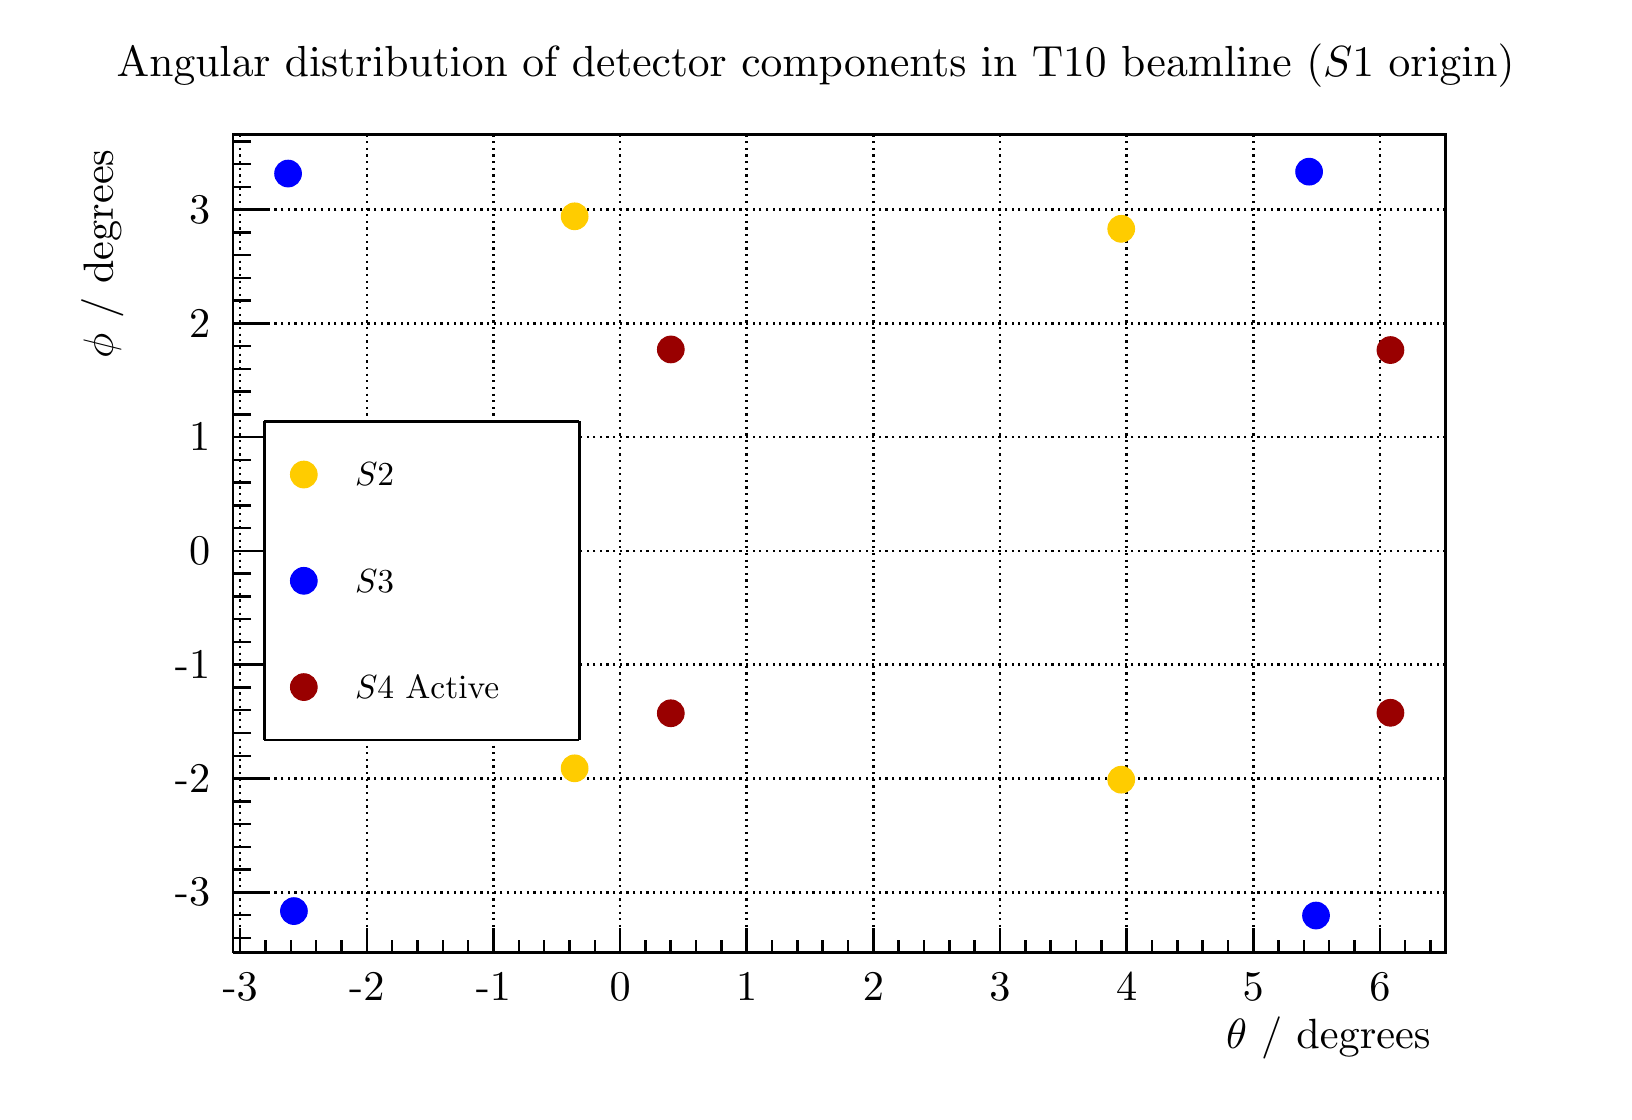
\begin{tikzpicture}
\pgfdeclareplotmark{cross} {
\pgfpathmoveto{\pgfpoint{-0.3\pgfplotmarksize}{\pgfplotmarksize}}
\pgfpathlineto{\pgfpoint{+0.3\pgfplotmarksize}{\pgfplotmarksize}}
\pgfpathlineto{\pgfpoint{+0.3\pgfplotmarksize}{0.3\pgfplotmarksize}}
\pgfpathlineto{\pgfpoint{+1\pgfplotmarksize}{0.3\pgfplotmarksize}}
\pgfpathlineto{\pgfpoint{+1\pgfplotmarksize}{-0.3\pgfplotmarksize}}
\pgfpathlineto{\pgfpoint{+0.3\pgfplotmarksize}{-0.3\pgfplotmarksize}}
\pgfpathlineto{\pgfpoint{+0.3\pgfplotmarksize}{-1.\pgfplotmarksize}}
\pgfpathlineto{\pgfpoint{-0.3\pgfplotmarksize}{-1.\pgfplotmarksize}}
\pgfpathlineto{\pgfpoint{-0.3\pgfplotmarksize}{-0.3\pgfplotmarksize}}
\pgfpathlineto{\pgfpoint{-1.\pgfplotmarksize}{-0.3\pgfplotmarksize}}
\pgfpathlineto{\pgfpoint{-1.\pgfplotmarksize}{0.3\pgfplotmarksize}}
\pgfpathlineto{\pgfpoint{-0.3\pgfplotmarksize}{0.3\pgfplotmarksize}}
\pgfpathclose
\pgfusepathqstroke
}
\pgfdeclareplotmark{cross*} {
\pgfpathmoveto{\pgfpoint{-0.3\pgfplotmarksize}{\pgfplotmarksize}}
\pgfpathlineto{\pgfpoint{+0.3\pgfplotmarksize}{\pgfplotmarksize}}
\pgfpathlineto{\pgfpoint{+0.3\pgfplotmarksize}{0.3\pgfplotmarksize}}
\pgfpathlineto{\pgfpoint{+1\pgfplotmarksize}{0.3\pgfplotmarksize}}
\pgfpathlineto{\pgfpoint{+1\pgfplotmarksize}{-0.3\pgfplotmarksize}}
\pgfpathlineto{\pgfpoint{+0.3\pgfplotmarksize}{-0.3\pgfplotmarksize}}
\pgfpathlineto{\pgfpoint{+0.3\pgfplotmarksize}{-1.\pgfplotmarksize}}
\pgfpathlineto{\pgfpoint{-0.3\pgfplotmarksize}{-1.\pgfplotmarksize}}
\pgfpathlineto{\pgfpoint{-0.3\pgfplotmarksize}{-0.3\pgfplotmarksize}}
\pgfpathlineto{\pgfpoint{-1.\pgfplotmarksize}{-0.3\pgfplotmarksize}}
\pgfpathlineto{\pgfpoint{-1.\pgfplotmarksize}{0.3\pgfplotmarksize}}
\pgfpathlineto{\pgfpoint{-0.3\pgfplotmarksize}{0.3\pgfplotmarksize}}
\pgfpathclose
\pgfusepathqfillstroke
}
\pgfdeclareplotmark{newstar} {
\pgfpathmoveto{\pgfqpoint{0pt}{\pgfplotmarksize}}
\pgfpathlineto{\pgfqpointpolar{44}{0.5\pgfplotmarksize}}
\pgfpathlineto{\pgfqpointpolar{18}{\pgfplotmarksize}}
\pgfpathlineto{\pgfqpointpolar{-20}{0.5\pgfplotmarksize}}
\pgfpathlineto{\pgfqpointpolar{-54}{\pgfplotmarksize}}
\pgfpathlineto{\pgfqpointpolar{-90}{0.5\pgfplotmarksize}}
\pgfpathlineto{\pgfqpointpolar{234}{\pgfplotmarksize}}
\pgfpathlineto{\pgfqpointpolar{198}{0.5\pgfplotmarksize}}
\pgfpathlineto{\pgfqpointpolar{162}{\pgfplotmarksize}}
\pgfpathlineto{\pgfqpointpolar{134}{0.5\pgfplotmarksize}}
\pgfpathclose
\pgfusepathqstroke
}
\pgfdeclareplotmark{newstar*} {
\pgfpathmoveto{\pgfqpoint{0pt}{\pgfplotmarksize}}
\pgfpathlineto{\pgfqpointpolar{44}{0.5\pgfplotmarksize}}
\pgfpathlineto{\pgfqpointpolar{18}{\pgfplotmarksize}}
\pgfpathlineto{\pgfqpointpolar{-20}{0.5\pgfplotmarksize}}
\pgfpathlineto{\pgfqpointpolar{-54}{\pgfplotmarksize}}
\pgfpathlineto{\pgfqpointpolar{-90}{0.5\pgfplotmarksize}}
\pgfpathlineto{\pgfqpointpolar{234}{\pgfplotmarksize}}
\pgfpathlineto{\pgfqpointpolar{198}{0.5\pgfplotmarksize}}
\pgfpathlineto{\pgfqpointpolar{162}{\pgfplotmarksize}}
\pgfpathlineto{\pgfqpointpolar{134}{0.5\pgfplotmarksize}}
\pgfpathclose
\pgfusepathqfillstroke
}
\definecolor{c}{rgb}{1,1,1};
\draw [color=c, fill=c] (0,0) rectangle (20,13.4957);
\draw [color=c, fill=c] (2.6,1.75444) rectangle (18,12.1461);
\definecolor{c}{rgb}{0,0,0};
\draw [c,line width=0.9] (2.6,1.75444) -- (2.6,12.1461) -- (18,12.1461) -- (18,1.75444) -- (2.6,1.75444);
\definecolor{c}{rgb}{1,1,1};
\draw [color=c, fill=c] (2.6,1.75444) rectangle (18,12.1461);
\definecolor{c}{rgb}{0,0,0};
\draw [c,line width=0.9] (2.6,1.75444) -- (2.6,12.1461) -- (18,12.1461) -- (18,1.75444) -- (2.6,1.75444);
\draw [c,line width=0.9] (2.6,1.75444) -- (18,1.75444);
\draw [c,dash pattern=on 0.80pt off 1.60pt ,line width=0.9] (2.69176,12.1461) -- (2.69176,1.75444);
\draw [c,dash pattern=on 0.80pt off 1.60pt ,line width=0.9] (4.30001,12.1461) -- (4.30001,1.75444);
\draw [c,dash pattern=on 0.80pt off 1.60pt ,line width=0.9] (5.90825,12.1461) -- (5.90825,1.75444);
\draw [c,dash pattern=on 0.80pt off 1.60pt ,line width=0.9] (7.5165,12.1461) -- (7.5165,1.75444);
\draw [c,dash pattern=on 0.80pt off 1.60pt ,line width=0.9] (9.12474,12.1461) -- (9.12474,1.75444);
\draw [c,dash pattern=on 0.80pt off 1.60pt ,line width=0.9] (10.733,12.1461) -- (10.733,1.75444);
\draw [c,dash pattern=on 0.80pt off 1.60pt ,line width=0.9] (12.3412,12.1461) -- (12.3412,1.75444);
\draw [c,dash pattern=on 0.80pt off 1.60pt ,line width=0.9] (13.9495,12.1461) -- (13.9495,1.75444);
\draw [c,dash pattern=on 0.80pt off 1.60pt ,line width=0.9] (15.5577,12.1461) -- (15.5577,1.75444);
\draw [c,dash pattern=on 0.80pt off 1.60pt ,line width=0.9] (17.166,12.1461) -- (17.166,1.75444);
\draw [c,dash pattern=on 0.80pt off 1.60pt ,line width=0.9] (2.69176,12.1461) -- (2.69176,1.75444);
\draw [c,dash pattern=on 0.80pt off 1.60pt ,line width=0.9] (17.166,12.1461) -- (17.166,1.75444);
\draw [c,line width=0.9] (2.6,1.75444) -- (2.6,12.1461);
\draw [c,dash pattern=on 0.80pt off 1.60pt ,line width=0.9] (18,2.52225) -- (2.6,2.52225);
\draw [c,dash pattern=on 0.80pt off 1.60pt ,line width=0.9] (18,3.9671) -- (2.6,3.9671);
\draw [c,dash pattern=on 0.80pt off 1.60pt ,line width=0.9] (18,5.41196) -- (2.6,5.41196);
\draw [c,dash pattern=on 0.80pt off 1.60pt ,line width=0.9] (18,6.85681) -- (2.6,6.85681);
\draw [c,dash pattern=on 0.80pt off 1.60pt ,line width=0.9] (18,8.30166) -- (2.6,8.30166);
\draw [c,dash pattern=on 0.80pt off 1.60pt ,line width=0.9] (18,9.74652) -- (2.6,9.74652);
\draw [c,dash pattern=on 0.80pt off 1.60pt ,line width=0.9] (18,11.1914) -- (2.6,11.1914);
\draw [c,dash pattern=on 0.80pt off 1.60pt ,line width=0.9] (18,2.52225) -- (2.6,2.52225);
\draw [c,dash pattern=on 0.80pt off 1.60pt ,line width=0.9] (18,11.1914) -- (2.6,11.1914);
\draw [c,line width=0.9] (2.6,1.75444) -- (18,1.75444);
\draw [c,line width=0.9] (2.69176,2.06619) -- (2.69176,1.75444);
\draw [c,line width=0.9] (3.01341,1.91032) -- (3.01341,1.75444);
\draw [c,line width=0.9] (3.33506,1.91032) -- (3.33506,1.75444);
\draw [c,line width=0.9] (3.65671,1.91032) -- (3.65671,1.75444);
\draw [c,line width=0.9] (3.97836,1.91032) -- (3.97836,1.75444);
\draw [c,line width=0.9] (4.30001,2.06619) -- (4.30001,1.75444);
\draw [c,line width=0.9] (4.62165,1.91032) -- (4.62165,1.75444);
\draw [c,line width=0.9] (4.9433,1.91032) -- (4.9433,1.75444);
\draw [c,line width=0.9] (5.26495,1.91032) -- (5.26495,1.75444);
\draw [c,line width=0.9] (5.5866,1.91032) -- (5.5866,1.75444);
\draw [c,line width=0.9] (5.90825,2.06619) -- (5.90825,1.75444);
\draw [c,line width=0.9] (6.2299,1.91032) -- (6.2299,1.75444);
\draw [c,line width=0.9] (6.55155,1.91032) -- (6.55155,1.75444);
\draw [c,line width=0.9] (6.8732,1.91032) -- (6.8732,1.75444);
\draw [c,line width=0.9] (7.19485,1.91032) -- (7.19485,1.75444);
\draw [c,line width=0.9] (7.5165,2.06619) -- (7.5165,1.75444);
\draw [c,line width=0.9] (7.83815,1.91032) -- (7.83815,1.75444);
\draw [c,line width=0.9] (8.15979,1.91032) -- (8.15979,1.75444);
\draw [c,line width=0.9] (8.48144,1.91032) -- (8.48144,1.75444);
\draw [c,line width=0.9] (8.80309,1.91032) -- (8.80309,1.75444);
\draw [c,line width=0.9] (9.12474,2.06619) -- (9.12474,1.75444);
\draw [c,line width=0.9] (9.44639,1.91032) -- (9.44639,1.75444);
\draw [c,line width=0.9] (9.76804,1.91032) -- (9.76804,1.75444);
\draw [c,line width=0.9] (10.0897,1.91032) -- (10.0897,1.75444);
\draw [c,line width=0.9] (10.4113,1.91032) -- (10.4113,1.75444);
\draw [c,line width=0.9] (10.733,2.06619) -- (10.733,1.75444);
\draw [c,line width=0.9] (11.0546,1.91032) -- (11.0546,1.75444);
\draw [c,line width=0.9] (11.3763,1.91032) -- (11.3763,1.75444);
\draw [c,line width=0.9] (11.6979,1.91032) -- (11.6979,1.75444);
\draw [c,line width=0.9] (12.0196,1.91032) -- (12.0196,1.75444);
\draw [c,line width=0.9] (12.3412,2.06619) -- (12.3412,1.75444);
\draw [c,line width=0.9] (12.6629,1.91032) -- (12.6629,1.75444);
\draw [c,line width=0.9] (12.9845,1.91032) -- (12.9845,1.75444);
\draw [c,line width=0.9] (13.3062,1.91032) -- (13.3062,1.75444);
\draw [c,line width=0.9] (13.6278,1.91032) -- (13.6278,1.75444);
\draw [c,line width=0.9] (13.9495,2.06619) -- (13.9495,1.75444);
\draw [c,line width=0.9] (14.2711,1.91032) -- (14.2711,1.75444);
\draw [c,line width=0.9] (14.5928,1.91032) -- (14.5928,1.75444);
\draw [c,line width=0.9] (14.9144,1.91032) -- (14.9144,1.75444);
\draw [c,line width=0.9] (15.2361,1.91032) -- (15.2361,1.75444);
\draw [c,line width=0.9] (15.5577,2.06619) -- (15.5577,1.75444);
\draw [c,line width=0.9] (15.8794,1.91032) -- (15.8794,1.75444);
\draw [c,line width=0.9] (16.201,1.91032) -- (16.201,1.75444);
\draw [c,line width=0.9] (16.5227,1.91032) -- (16.5227,1.75444);
\draw [c,line width=0.9] (16.8443,1.91032) -- (16.8443,1.75444);
\draw [c,line width=0.9] (17.166,2.06619) -- (17.166,1.75444);
\draw [c,line width=0.9] (2.69176,2.06619) -- (2.69176,1.75444);
\draw [c,line width=0.9] (17.166,2.06619) -- (17.166,1.75444);
\draw [c,line width=0.9] (17.4876,1.91032) -- (17.4876,1.75444);
\draw [c,line width=0.9] (17.8093,1.91032) -- (17.8093,1.75444);
\draw [anchor=base] (2.69176,1.14713) node[scale=1.52731, color=c, rotate=0]{-3};
\draw [anchor=base] (4.30001,1.14713) node[scale=1.52731, color=c, rotate=0]{-2};
\draw [anchor=base] (5.90825,1.14713) node[scale=1.52731, color=c, rotate=0]{-1};
\draw [anchor=base] (7.5165,1.14713) node[scale=1.52731, color=c, rotate=0]{0};
\draw [anchor=base] (9.12474,1.14713) node[scale=1.52731, color=c, rotate=0]{1};
\draw [anchor=base] (10.733,1.14713) node[scale=1.52731, color=c, rotate=0]{2};
\draw [anchor=base] (12.3412,1.14713) node[scale=1.52731, color=c, rotate=0]{3};
\draw [anchor=base] (13.9495,1.14713) node[scale=1.52731, color=c, rotate=0]{4};
\draw [anchor=base] (15.5577,1.14713) node[scale=1.52731, color=c, rotate=0]{5};
\draw [anchor=base] (17.166,1.14713) node[scale=1.52731, color=c, rotate=0]{6};
\draw [anchor= east] (18,0.674785) node[scale=1.52731, color=c, rotate=0]{$\theta$ / degrees};
\draw [c,line width=0.9] (2.6,1.75444) -- (2.6,12.1461);
\draw [c,line width=0.9] (3.062,2.52225) -- (2.6,2.52225);
\draw [c,line width=0.9] (2.831,2.81122) -- (2.6,2.81122);
\draw [c,line width=0.9] (2.831,3.10019) -- (2.6,3.10019);
\draw [c,line width=0.9] (2.831,3.38916) -- (2.6,3.38916);
\draw [c,line width=0.9] (2.831,3.67813) -- (2.6,3.67813);
\draw [c,line width=0.9] (3.062,3.9671) -- (2.6,3.9671);
\draw [c,line width=0.9] (2.831,4.25607) -- (2.6,4.25607);
\draw [c,line width=0.9] (2.831,4.54504) -- (2.6,4.54504);
\draw [c,line width=0.9] (2.831,4.83401) -- (2.6,4.83401);
\draw [c,line width=0.9] (2.831,5.12298) -- (2.6,5.12298);
\draw [c,line width=0.9] (3.062,5.41196) -- (2.6,5.41196);
\draw [c,line width=0.9] (2.831,5.70093) -- (2.6,5.70093);
\draw [c,line width=0.9] (2.831,5.9899) -- (2.6,5.9899);
\draw [c,line width=0.9] (2.831,6.27887) -- (2.6,6.27887);
\draw [c,line width=0.9] (2.831,6.56784) -- (2.6,6.56784);
\draw [c,line width=0.9] (3.062,6.85681) -- (2.6,6.85681);
\draw [c,line width=0.9] (2.831,7.14578) -- (2.6,7.14578);
\draw [c,line width=0.9] (2.831,7.43475) -- (2.6,7.43475);
\draw [c,line width=0.9] (2.831,7.72372) -- (2.6,7.72372);
\draw [c,line width=0.9] (2.831,8.01269) -- (2.6,8.01269);
\draw [c,line width=0.9] (3.062,8.30166) -- (2.6,8.30166);
\draw [c,line width=0.9] (2.831,8.59064) -- (2.6,8.59064);
\draw [c,line width=0.9] (2.831,8.87961) -- (2.6,8.87961);
\draw [c,line width=0.9] (2.831,9.16858) -- (2.6,9.16858);
\draw [c,line width=0.9] (2.831,9.45755) -- (2.6,9.45755);
\draw [c,line width=0.9] (3.062,9.74652) -- (2.6,9.74652);
\draw [c,line width=0.9] (2.831,10.0355) -- (2.6,10.0355);
\draw [c,line width=0.9] (2.831,10.3245) -- (2.6,10.3245);
\draw [c,line width=0.9] (2.831,10.6134) -- (2.6,10.6134);
\draw [c,line width=0.9] (2.831,10.9024) -- (2.6,10.9024);
\draw [c,line width=0.9] (3.062,11.1914) -- (2.6,11.1914);
\draw [c,line width=0.9] (3.062,2.52225) -- (2.6,2.52225);
\draw [c,line width=0.9] (2.831,2.23328) -- (2.6,2.23328);
\draw [c,line width=0.9] (2.831,1.9443) -- (2.6,1.9443);
\draw [c,line width=0.9] (3.062,11.1914) -- (2.6,11.1914);
\draw [c,line width=0.9] (2.831,11.4803) -- (2.6,11.4803);
\draw [c,line width=0.9] (2.831,11.7693) -- (2.6,11.7693);
\draw [c,line width=0.9] (2.831,12.0583) -- (2.6,12.0583);
\draw [anchor= east] (2.5,2.52225) node[scale=1.52731, color=c, rotate=0]{-3};
\draw [anchor= east] (2.5,3.9671) node[scale=1.52731, color=c, rotate=0]{-2};
\draw [anchor= east] (2.5,5.41196) node[scale=1.52731, color=c, rotate=0]{-1};
\draw [anchor= east] (2.5,6.85681) node[scale=1.52731, color=c, rotate=0]{0};
\draw [anchor= east] (2.5,8.30166) node[scale=1.52731, color=c, rotate=0]{1};
\draw [anchor= east] (2.5,9.74652) node[scale=1.52731, color=c, rotate=0]{2};
\draw [anchor= east] (2.5,11.1914) node[scale=1.52731, color=c, rotate=0]{3};
\draw [anchor= east] (0.940974,12.1461) node[scale=1.52731, color=c, rotate=90]{$\phi$ / degrees};
\definecolor{c}{rgb}{1,0.8,0};
\foreach \P in {(6.93952,11.107), (6.93952,4.09655), (13.8811,3.95207), (13.8811,10.948)}{\draw[mark options={color=c,fill=c},mark size=4.804805pt,mark=*] plot coordinates {\P};}
\definecolor{c}{rgb}{0,0,1};
\foreach \P in {(3.3,11.6499), (16.2669,11.6738), (3.37447,2.28348), (16.3549,2.22679)}{\draw[mark options={color=c,fill=c},mark size=4.804805pt,mark=*] plot coordinates {\P};}
\definecolor{c}{rgb}{0.6,0,0};
\foreach \P in {(8.16076,9.41611), (17.3,9.40847), (8.16076,4.79569), (17.3,4.80184)}{\draw[mark options={color=c,fill=c},mark size=4.804805pt,mark=*] plot coordinates {\P};}
\definecolor{c}{rgb}{1,1,1};
\draw [color=c, fill=c] (3,4.45358) rectangle (7,8.50229);
\definecolor{c}{rgb}{0,0,0};
\draw [c,line width=0.9] (3,4.45358) -- (7,4.45358);
\draw [c,line width=0.9] (7,4.45358) -- (7,8.50229);
\draw [c,line width=0.9] (7,8.50229) -- (3,8.50229);
\draw [c,line width=0.9] (3,8.50229) -- (3,4.45358);
\draw [anchor= west] (4,7.82751) node[scale=1.20912, color=c, rotate=0]{$S2$};
\definecolor{c}{rgb}{1,0.8,0};
\foreach \P in {(3.5,7.82751)}{\draw[mark options={color=c,fill=c},mark size=4.804805pt,mark=*] plot coordinates {\P};}
\definecolor{c}{rgb}{0,0,0};
\draw [anchor= west] (4,6.47794) node[scale=1.20912, color=c, rotate=0]{$S3$};
\definecolor{c}{rgb}{0,0,1};
\foreach \P in {(3.5,6.47794)}{\draw[mark options={color=c,fill=c},mark size=4.804805pt,mark=*] plot coordinates {\P};}
\definecolor{c}{rgb}{0,0,0};
\draw [anchor= west] (4,5.12837) node[scale=1.20912, color=c, rotate=0]{$S4$ Active};
\definecolor{c}{rgb}{0.6,0,0};
\foreach \P in {(3.5,5.12837)}{\draw[mark options={color=c,fill=c},mark size=4.804805pt,mark=*] plot coordinates {\P};}
\definecolor{c}{rgb}{0,0,0};
\draw (10,13.0156) node[scale=1.5731, color=c, rotate=0]{Angular distribution of detector components in T10 beamline ($S1$ origin)};
\end{tikzpicture}
